\section{Deterministic State Generator}

As PRISM-games was insufficient (refer to \cref{section:prism-results} ) for verifying the equality of the game, a custom modeller was created in an attempt to verify the game through a different technique. The deterministic state generator mimics the functionality of PRISM-games, generating the set of all possible states and transitions. In addition, querying paths and reachability can be tailored to the custom implementation rather than conform to PRISM-games property syntax.

\subsection{Parameterisation}

The state generator accepts the following as parameters as a basis to creating states:

\begin{itemize}
    \item $r$ - Tax rate.
    \item $d$ - Discount factor.
    \item $R$ - Expected reward per owned chunk.
    \item $t$ - Threshold at which to consider the reward as too low.
\end{itemize}

For the purposes of modelling, each participant is represented by an object with the following properties:

\begin{itemize}
    \item $balance$ - the current value in the participants possession as a unit of the block reward.
    \item $chunks$ - the current number of chunks in the participants possession.
    \item $chance$ - A chance used to determine if a participant will participate, initiate an auction, or withhold.
\end{itemize}

Each state created in the state generator can be defined as:

\begin{align}
    S :=&\; (c, d, a, P) \\
    P =&\; \{p_0, p_1, \ldots, p_n\}
\end{align}

\noindent Where the parameters are as follows
\begin{itemize}
    \item $c$ - The probability of reaching this state. Refer to \cref{equation:stateprobability} below.
    \item $d$ - The number of steps to reach this state (or depth).
    \item $a$ - The action taken to transition to this state.
    \item $P$ - A set of participant objects containing their initial state.
\end{itemize}

Each state represents the funds and chunks of each participant and maintains a reference to future states. Algorithm \ref{algorithm:generatestates} details the recursive process of generating states.

An action represents the decision made by one or many participants to change the current state or by the distribution of a reward. It may be represented as:

\begin{align}
    A :=&\; (\tau, c, S_t) \\
    S_t =&\; {t_0, t_1, \ldots, t_n} \\
    \tau \in&\; \{\textsc{Reward, Purchase}\}
\end{align}

\noindent Where the parameters are as follows
\begin{itemize}
    \item $\tau$ - The transition type.
    \item $c$ - The probability of this transition occurring. Refer to \crefrange{equation:participantactions}{equation:participantactionsend} below.
    \item $S_t$ - The set of transactions executed in this transition. Zero or more discrete transactions such that $\forall t \in S_t : \nexists \; t' \in S_t : t.buyer = t'.buyer$.
\end{itemize}

A transaction contains details about the transferal of chunk ownership between participants and can be defined as the following:

\begin{equation}
    T := (b, s, p)
\end{equation}

\noindent Where the parameters are as follows
\begin{itemize}
    \item $b$ - The buyer who initiated the transaction.
    \item $s$ - The seller from which the chunk will be transferred from.
    \item $p$ - The price at which the buyer is purchasing for.
\end{itemize}

\subsection{Modelling}

In order to facilitate the modelling of the game as a Markov chain, the probability of a participants actions can be defined on set of participants $P$ and the above parameters:

\begin{align} \label{equation:participantactions}
    \forall b \in Buyers &: b.chance > 0 \land b.funds \geq 1 \\
    \forall s \in Sellers &: b.chunks \geq 1 \\
    P(b_{purchase}) &= \frac{b.chance}{Sellers.length} \label{equation:probabilitypurchase}\\
    f(s) &= \label{equation:participantactionsend}
        \begin{cases}
            P(b_{purchase})     & \text{if $b$ chooses to purchase} \\
            P(1 - b_{purchase}) & \text{else if $b$ can purchase but chooses to withhold} \\
            1                   & \text{else if $b$ has insufficient funds to purchase}
        \end{cases}
\end{align}

The probability of reaching a state $X$ may then be calculated as the product of actions taken to reach it:

\begin{equation}
    P(X) = P(X_{prev}) \times \prod_{i=1}^{Buyers} action(b_i) \label{equation:stateprobability}
\end{equation}

The expected reward may then be calculated using the product of the balances at each end state and the state probability. Given a set of end states $\{X_{x \mid 0}, X_{x \mid 1}, \ldots, X_{x \mid n}\}$, where $X_{x \mid i}$ represents the balance of participant $x$ at the $i$th state $X$. Hence for participant $x$, the expected reward can be calculated as:

\begin{equation} \label{algorithm:state-expected-reward}
    \mathbb{E}(R(x \mid i)) = \sum_{i = 0}^n X_{x \mid i} \times P(X_{x \mid i})
\end{equation}

\subsection{Algorithms}

The following algorithms should be the minimum required logic in order to create a Deterministic State Generator according to the above game specifications detailed in previous sections.

Algorithm \ref{algorithm:generatestates} below shows the process for which states were recursively generated. A new state is created for each potential combination or subset of possible transactions the participants are able to take in the current state until no more actions can be taken or the reward is reduced below a threshold due to the discount factor. It accepts the following parameters:

\begin{itemize}
    \item $S_\rho$ - The set of participants.
    \item $state$ - The new state.
    \item $depth$ - The current depth.
\end{itemize}

\begin{algorithm}[H]
\caption{Recursive state generator}
\label{algorithm:generatestates}
\begin{algorithmic}[1]
\Procedure{generateStates}{$S_\rho, state, depth$}
    \State $r \gets R(depth)$ \Comment{refer to \cref{equation:rewarddiscounted}}
    \If{$r < t$}
        \State \Return
    \EndIf
    \State $state.subStates \gets \textsc{empty set of State}$
    \State $S_t \gets \textsc{generateTransactions}(S_\rho)$ \Comment{refer to \cref{algorithm:generatetransactions}}
    \State $S_c \gets \textsc{calculateStateChance}(state, S_t, S_\rho)$ \Comment{refer to \cref{algorithm:calculatestatechance}}
    \For{$i \in [0, S_t.length)$}
        \State $action \gets new \textsc{ Action}(S_t[i], S_c[i])$
        \State $S_\rho' \gets \textsc{applyAction}(S_\rho, action)$ \Comment{refer to \cref{algorithm:applyaction}}
        \State $subState \gets new \textsc{ State}(S_\rho', action)$
        \State $state.subStates \gets state.subStates \cup \{subState\}$
        \State $\textsc{generateStates}(S_\rho', subState, depth + 1)$
    \EndFor
\EndProcedure
\end{algorithmic}
\end{algorithm}

Algorithm \ref{algorithm:generatetransactions} generates all possible combinations and subsets of transactions given the current participants state. It accepts the set of participants $S_\rho$ as the basis for determining possible transactions.

\begin{algorithm}[H]
\caption{Transaction combination generator}
\label{algorithm:generatetransactions}
\begin{algorithmic}[1]
\Procedure{generateTransactions}{$S_\rho$}
    \State $B \gets \{ b \in S_\rho \mid b.balance \geq 1 \land b.chance > 0 \}$
    \State $S \gets \{ s \in S_\rho \mid s.chunks \geq 1 \}$
    \State $transactionSets \gets \textsc{empty set of set of Transaction}$
    \For{$b \in B$}
        \State $set \gets \textsc{empty set of Transaction}$
        \For{$s \in S$}
            \State $set \gets set \cup \{new \textsc{ Transaction}(b, s)\}$
        \EndFor
        \State $transactionSets \gets transactionSets \cup \{set\}$
    \EndFor
    \State $result \gets \textsc{empty set of set of Transaction}$
    \State $unvisited \gets TransactionSets$
    \While{$unvisited \neq \emptyset$}
        \State $set \gets unvisited.\textsc{pop}()$
        \For{$transaction \in set$}
            \For{$otherSet \in unvisited$}
                \For{$otherTransaction \in otherSet$}
                    \If{$transaction.seller \neq otherTransaction.seller$
                        \State $\lor \; transaction.seller.chunks > 1$}
                        \State $result \gets result \cup \{[transaction, otherTransaction]\}$
                    \EndIf
                \EndFor
            \EndFor
            \State $result \gets result \cup \{[transaction]\}$
        \EndFor
    \EndWhile
    \State \Return $result$
\EndProcedure
\end{algorithmic}
\end{algorithm}

Algorithm \ref{algorithm:calculatestatechance} below determines the probability distribution of states belonging to a parent state. It considers all participants with the ability to purchase and determines the probability of each action occurring. Participants who are not in the set $B$ defined in line 2 are considered to not be eligible for purchasing and are not considered as they would not have a choice. The algorithm accepts the following parameters: 

\begin{itemize}
    \item $T$ - The set of transitional transactions.
    \item $S_\rho$ - The set of participants.
\end{itemize}

\begin{algorithm}[H]
\caption{Determines the chance of a state given a transition and parent state. }
\label{algorithm:calculatestatechance}
\begin{algorithmic}[1]
\Procedure{calculateStateChance}{$T, S_\rho$} 
    \State $B \gets \{ b \in S_\rho \mid b.balance \geq 1 \land b.chance > 0 \}$
    \State $S \gets \{ s \in S_\rho \mid s.chunks \geq 1 \}$
    \State $chances \gets 1$
    \For{$b \in B$}
        \If{$t \in T : t.buyer = b$}
            \State $chances \gets chances \times \frac{b.chance}{length(S - b)}$
        \Else
            \State $chances \gets chances \times (1 - b.chance)$
        \EndIf
    \EndFor
    \State $total \gets 1$
    \State \Return $chances$
\EndProcedure
\end{algorithmic}
\end{algorithm}

Algorithm \ref{algorithm:applyaction} below updates the state of each participant to apply a transition to the state owning the given set of participants. It accepts the following parameters:

\begin{itemize}
    \item $S_\rho$ - The set of participants.
    \item $a$ - The transitional action to apply to the state
\end{itemize}

\begin{algorithm}[H]
\caption{Applies a transition on a state}
\label{algorithm:applyaction}
\begin{algorithmic}[1]
\Procedure{applyAction}{$S_\rho, a$}
    \Switch{$a.\tau$}
        \Case \textsc{Reward}
            \For{$\rho \in S_\rho$}
                \State $\rho.funds \gets \rho.funds + R(\rho.chunks)$ \Comment{refer to \cref{equation:rewarddiscounted}}
            \EndFor
        \EndCase
        \Case \textsc{Purchase}
            \For{$t \in action.S_t$}
                \State $t.buyer.funds \gets t.buyer.funds - t.price$
                \State $t.buyer.chunks \gets t.buyer.chunks + 1$
                \State $t.seller.funds \gets t.seller.funds + t.price$
                \State $t.seller.chunks \gets t.seller.chunks - 1$
            \EndFor
        \EndCase
    \EndSwitch
\EndProcedure
\end{algorithmic}
\end{algorithm}

\subsection{Implementation}

The source code for the implementation used for the purposes of this project can be found on Gitlab \footnote{\url{https://gitlab.com/harberger-tax/state-diagram-generator}}. Created in TypeScript \cite{typescript2020}, it provides a command line interface with a number of options to programmatically change how the resultant states are generated. 

The program was created in TypeScript due to familiarity and syntactical convenience, with fast prototyping and compilation, it was preferable for fast prototyping. In addition to the generator, a visualisation utility was added utilising Mermaid \cite{mermaid} which enabled rendering smaller scale state diagrams for visual inspection. Additionally, as it is natively supported in all browsers, it is trivial to embed functionality into other projects such as the demonstration (refer to \cref{section:demonstration}). With the system used for experimentation in \cref{appendix:computerspecs}, a maximum depth of 30 yielded over 2.5 million states in ~40 seconds and utilising over 5GB of ram. At a discount factor of 0.01, a tax rate of 0.05, and a threshold of 0.009, the maximum depth required at 4713 would not be feasible as the amount of memory required to create the complete set states far exceed the computational resources available.

Figure \ref{figure:state-diagram-small} below shows a small sample set of states generated with participants having a chance of 0.9 and a maximum depth of 1. Each node contains information on the current state of each participant in the form P$i$: $c$, $f$ where $i$ is the ID of the participant, $c$ is the owned chunks, and $f$ is the current balance. Each arrow represents a transition in which either the distribution of chunks or funds of any participant observes a change and are labelled with the chance for the transition to occur and the reason for the transition (A purchase, reward, or no change occurred).

\begin{figure}[H]
  \centering
  \caption{Deterministic state generator minimal example}
  \label{figure:state-diagram-small}
  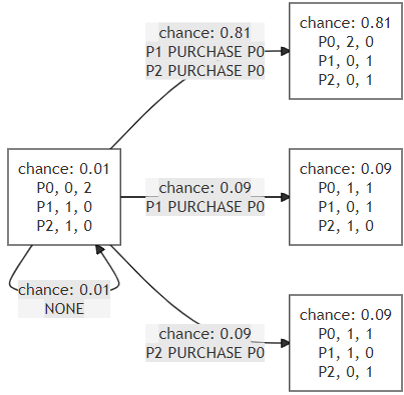
\includegraphics[width=0.5\textwidth]{media/state-diagram-small.PNG}
\end{figure}
